\newpage
\begin{center}
  \textbf{\large 3. ВНЕДРЕНИЕ И ЭКСПЛУАТАЦИЯ}
\end{center}
\refstepcounter{chapter}
\addcontentsline{toc}{chapter}{3. ВНЕДРЕНИЕ И ЭКСПЛУАТАЦИЯ}



\section{Развертывание платформы в среде Kubernetes}

Важным аспектом разработки информационной системы является правильное размещение готовго решения на целевой инфораструктуре. При выборе конфигурации серверного оборудования важно учитывать архитектурные особенности разработанной системы. В текущем разделе работы предствлены сведения об архитектуре развертывания приложения, требования к низлежащей инфраструктуре кластера Kubernetes, описание процесс установки основных компонентов платформы.

\subsection{Диаграмма развертывания}

Вся разработанная система развертывается в Kubernetes. Это обеспечивает отказоустойчивасть, масштабируемость, а так же возможность использования большого колличества серверов для развертывания пользовательских задач. 

Высокоурованевая диаграмма развертывания компонентов системы представлена на рисунке ~\ref{deploy}.

\begin{figure*}[!t]
  \centering
  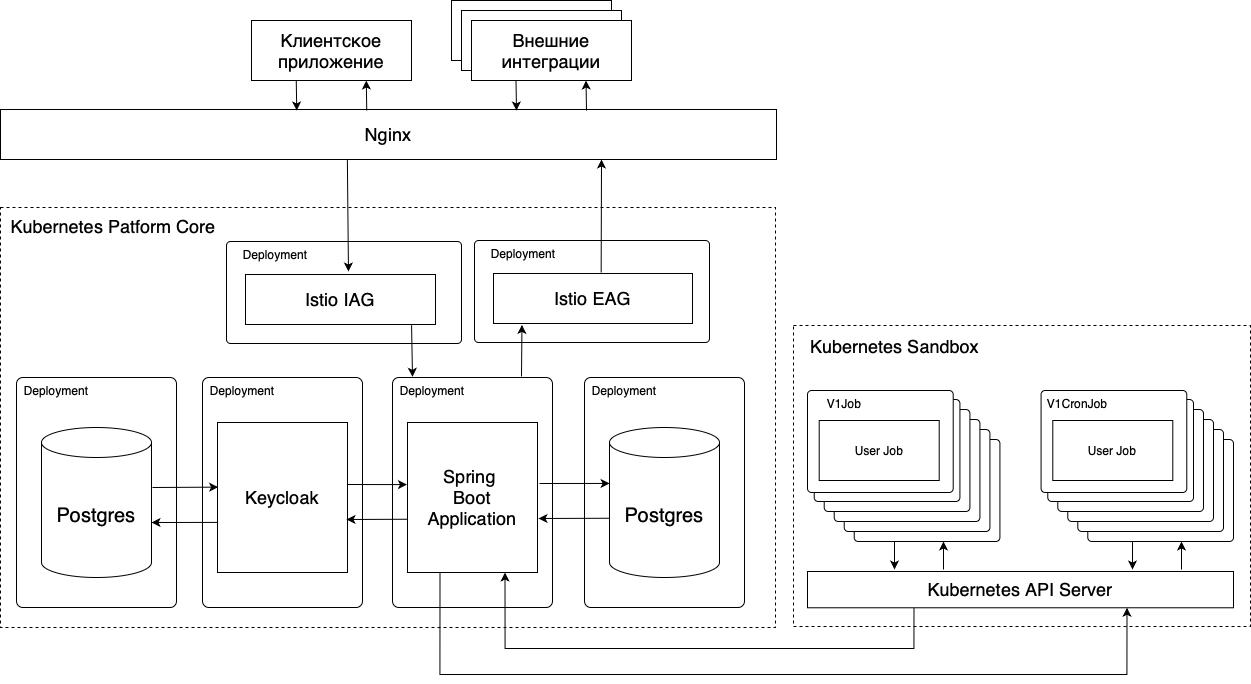
\includegraphics[width=\linewidth]{generated/deploy.drawio.png}
  \caption{Диаграмма развертывания}
  \label{deploy}
\end{figure*}

Все ключевые компоненты системы разворачиваются в $platform-core$ нэймспейсе и каждый представляет собой отдельный Deployment компонент Kubernetes.
В то же время пользовательские компоненты разворачиваются в изолированой среде $sandbox$ и являются объектами $V1Job$ и $V1CronJob$ в зависимости от конфигурации компонента.

Внешний пользовательский трафик поступает в систему через обратный прокси Nginx, который в тоже же время является SSL-терминатором\cite{boisrond2020terminate} и корнем раздачи статических файлов.

\subsection{Требования к инфраструктуре}

Для успешного развертывания и функционирования автоматизированной платформы развертывания контейнеризованных функций необходимо обеспечить соответствие инфраструктуры следующим требованиям:

\subsubsection{Кластер Kubernetes}

Требуется наличие функционирующего кластера Kubernetes. Для использования всех возможностей и обеспечения совместимости с актуальными API рекомендуется версия 1.25 или выше.

Кластер должен иметь стандартную конфигурацию с работающими компонентами Control Plane (API Server, etcd, Scheduler, Controller Manager) и Worker Nodes (Kubelet, Kube-proxy, Container Runtime).

Серверное приложение платформы должно иметь права доступа к API Kubernetes для управления ресурсами (Jobs, CronJobs, Pods, Logs) в выделенном пространстве имен \texttt{sandbox}.

\subsubsection{Ресурсы узлов кластера}

Требования к ресурсам зависят от ожидаемой нагрузки: количества одновременно работающих пользовательских задач, их ресурсоемкости, а также активности пользователей платформы.

Минимальные требования к рабочему узлу для базового развертывания без значительной нагрузки:

\begin{itemize}
    \item[---] Backend: \textasciitilde 1 CPU, \textasciitilde 1-2 GiB RAM
    \item[---] Keycloak: \textasciitilde 1 CPU, \textasciitilde 1-2 GiB RAM (может требовать больше при большой базе пользователей/сессий)
    \item[---] PostgreSQL: \textasciitilde 1 CPU, \textasciitilde 1-2 GiB RAM (+ дисковое пространство)
    \item[---] Пользовательские задачи (\texttt{sandbox}): Ресурсы зависят от самих задач. Необходимо предусмотреть достаточный запас на узлах для их запуска.
\end{itemize}

Необходимо проводить нагрузочное тестирование для определения оптимальных лимитов и запросов ресурсов (requests/limits) для подов платформы и планировать ресурсы узлов с запасом.

\subsubsection{Доступ к образам контейнеров:}

Узлы кластера Kubernetes должны иметь сетевой доступ к реестру контейнеров Docker Hub, где хранятся образы Backend, Frontend и базовые образы для пользовательских задач.

\subsection{Процесс развертывания компонентов}

Развертывание платформы осуществляется в среде Kubernetes и базируется на применении манифестов, поставляемых в составе релизного дистрибутива, описывающих требуемое состояние системы.

Процесс включает последовательное создание и настройку всех необходимых ресурсов Kubernetes для запуска основных компонентов платформы, таких как серверное приложение, система аутентификации, база данных, а также настройку сетевого взаимодействия и подготовку изолированного окружения (\texttt{sandbox}) для выполнения пользовательских задач.

Ниже описаны основные шаги, необходимые для развертывания каждого из ключевых компонентов.

\subsubsection{Развертывание серверной части (Backend)}

Развертывание серверной части, является ключевым шагом, так как этот компонент содержит основную бизнес-логику платформы. Процесс включает подготовку исполняемого артефакта, его контейнеризацию и последующее развертывание в кластере Kubernetes.

\subsubsection{Сборка приложения и упаковка в Docker-образ.}

Первым шагом является сборка приложения с использованием системы сборки Gradle. Команда сборки \texttt{./gradlew build} создает исполняемый JAR-файл в директории \texttt{build/libs}.

Далее, на основе этого JAR-файла и \texttt{Dockerfile}, создается Docker-образ приложения.

После создания образ загружается в реестр контейнеров, доступный для кластера Kubernetes. Этот процесс может быть выполен в ручную, так и автоматизирован в Ci/CD паплайне.

\subsubsection{Подготовка Kubernetes-манифестов.}

Для развертывания Backend в Kubernetes используются следующие основные типы манифестов:

\begin{itemize}
    \item[---]\textbf{Secret:} Используется для хранения чувствительных данных, таких как пароли и приватные ключи.
    \item[---]\textbf{ConfigMap:} Используется для хранения нечувствительной конфигурации в виде пар ключ-значение. 
    \item[---]\textbf{Deployment:} Основной манифест, описывающий желаемое состояние для подов Backend приложения.
    \item[---]\textbf{Service:} Определяет способ доступа к подам Backend внутри кластера.
\end{itemize}

\begin{lstlisting}[caption={Манифест Deployment компонета}, label=lst:manifest_example]
  apiVersion: apps/v1
  kind: Deployment
  metadata:
    name: backend-app          
    namespace: platform-core   
    labels:
      app: backend             
  spec:
    replicas: 2                
    selector:
      matchLabels:
        app: backend           
    template:
      metadata:
        labels:
          app: backend         
      spec:
        serviceAccountName: backend-service-account 
        containers:
          - name: backend-container 
            image: platform-registry/backend-app:latest 
            ports:
              - containerPort: 8080 
            envFrom:
              - configMapRef:
                  name: backend-config 
              - secretRef:
                  name: backend-secrets 
            resources:
              requests: 
                memory: "1Gi"
                cpu: "500m" 
              limits:   
                memory: "2Gi"
                cpu: "1"    
\end{lstlisting}

В листинге \ref{lst:manifest_example} предаствлен пример манифеста разворачиваемого Java приложения. Манифесты других компонентов идентичны и представлены в исходном коде разработанной системы.

\subsubsection{Применение манифестов.}

После подготовки всех YAML-файлов манифестов они применяются к кластеру Kubernetes с помощью команды:

\begin{verbatim}
kubectl apply -f <директория_с_манифестами> -n platform-core
\end{verbatim}

Kubernetes создаст необходимые объекты, скачает Docker-образ и запустит поды Backend приложения в соответствии с описанием в Deployment.

После успешного запуска подов и прохождения readiness-проб, Service начнет направлять трафик на них. На этом этапе серверная часть готова к приему запросов от Frontend или других компонентов системы. 

\subsubsection{Развертывание клиентской части (Frontend)}

Клиентская часть платформы, разработанная на Vue3, представляет собой одностраничное приложение (SPA), которое взаимодействует с пользователем и отправляет запросы к API серверной части. 

Развертывание Frontend включает сборку статических ассетов и их размещение на веб-сервере, доступном для пользователей.

Исходный код Vue3 приложения компилируется в набор статических файлов (HTML, CSS, JavaScript) с помощью инструментов сборки, таких как  Vite или Vue CLI. Сборка запускается командой \texttt{npm run build}.

Результат сборки (директория \texttt{dist}) содержит все необходимые файлы для работы приложения в браузере.

Для обслуживания статических файлов Frontend в Kubernetes использован веб-сервер Nginx, который раздает статические файлы потребителям.

\subsubsection{Инициализация базы данных}

После развертывания экземпляра PostgreSQL и перед полноценным запуском серверной части, необходимо инициализировать схему базы данных. Это включает создание таблиц, индексов, внешних ключей.

В разработанной системе для управления схемой базы данных используется инструмент миграций Liquibase. Этот инструмент интегрирован в Spring Boot приложение и позволяет версионировать изменения схемы БД и автоматически применять их при старте приложения.

Сервер авторизации Keycalok так же использует Liquibase для организации миграций базы данных.

Мигарции Liquibase поставляются вместе с дистрибутивом приложении и применяются при его запуске.

При последующих запусках пода Backend или при развертывании новых версий приложения с новыми скриптами миграций Liquibase будет применять только те миграции, которые еще не были выполнены, обеспечивая консистентность схемы БД.

\section{Реализация нефункциональных требований}
% Описание раздела: В данном разделе детально рассматривается, каким образом в архитектуре и реализации платформы были учтены ключевые нефункциональные требования, такие как безопасность, масштабируемость и отказоустойчивость.

Помимо реализации заявленной функциональности, описанной в предыдущих разделах, для создания надежной и эффективной системы критически важно уделить внимание нефункциональным требованиям (НФТ). 

В рамках разработки особое внимание было уделено трем нефункциональным требованиям: безопасности, масштабируемости и отказоустойчивости. Выбор архитектурных решений, стека технологий и конкретных механизмов реализации был во многом продиктован необходимостью обеспечения этих качеств.

\subsection{Обеспечение безопасности}

Безопасность крайне важна, поскольку система предполагает выполнение произвольного пользовательского кода, управляет доступом к ресурсам и обрабатывает пользовательские данные. В данном подразделе рассматриваются механизмы и решения, внедренные для минимизации рисков рисков безопасности.

\subsubsection{Аутентификация и авторизация}

Для реализации механизмов аутентификации и авторизации используется внешний сервер идентификации Keycloak, интегрированный с серверным приложением посредством стандартов OAuth 2.0 и OpenID Connect. Backend, выступая в роли Resource Server, отвечает за валидацию JWT-токенов доступа, получаемых от Keycloak, извлечение информации о пользователе и его ролях, а также за принудительное применение правил авторизации на уровне API эндпоинтов и отдельных операций с использованием возможностей фреймворка Spring Security.

Использование готовых решений и протоколов минимизирует риски возникнования ошибок при реализации механизмов аутентификации.

\subsubsection{Изоляция выполнения задач}

Поскольку платформа предназначена для запуска ппроизвольного пользовательского кода, критически важно предотвратить любое нежелательное взаимодействие этого кода с компонентами ядра системы или с кодом других пользователей. Для достижения этой цели реализован механизм строгой изоляции на уровне оркестратора Kubernetes, ключевым элементом которого является выделенное, логически обособленное пространство имен.

Все пользовательские задания, создаваемые платформой в виде объектов \texttt{Job} или \texttt{CronJob}, выполняются исключительно в пределах этого изолированного окружения, что фундаментально ограничивает их область видимости и потенциальное воздействие на остальную инфраструктуру кластера.

\subsection{Масштабируемость и производительность}

Способность платформы эффективно обрабатывать возрастающие нагрузки и обеспечивать быстрый отклик API являются ключевыми нефункциональными требованиями для ее успешной эксплуатации.

Использование Kubernetes в качестве среды развертывания предоставляет возможности для горизонтального масштабирования как компонентов самой платформы, так и ресурсов, выделяемых для выполнения пользовательских задач, позволяя динамически адаптироваться к изменениям нагрузки и обеспечивать стабильную работу системы.

\subsubsection{Горизонтальное масштабирование компонентов}

Серверная часть является stateless приложением и развертывается с использованием объекта Deployment. 
Этот объект позволяет декларативно управлять количеством работающих экземпляров каждого компонента через параметр \texttt{spec.replicas}.

При возрастании нагрузки администратор кластера может вручную увеличить количество реплик для Backend и других компонентов платформы, и Kubernetes автоматически запустит дополнительные поды, а Service (или Ingress) обеспечит распределение входящих запросов между всеми доступными экземплярами, повышая таким образом пропускную способность и отказоустойчивость сервиса.

\section{Тестирование платформы}

Тестирование позволяет выявить ошибки, узкие места и несоответствия на ранних стадиях, что существенно снижает затраты на их исправление и повышает общее качество конечного продукта. 

На текущем этапе проект находится в стадии активного прототипирования и разработки. В связи с этим, API платформы и внутренняя структура компонентов подвержены частым изменениям. По этой причине было принято решение временно отказаться от реализации полного покрытия кода модульными (unit) и интеграционными тестами. В условиях нестабильного API и быстрого развития функциональности, затраты на постоянную поддержку тестовой базы превысили бы получаемую пользу, замедляя процесс разработки прототипа. 

Было проведено ручное функциональное тестирование для проверки корректности работы ключевых аспектов платформы. Это тестирование охватывало как прямое взаимодействие с программным интерфейсом (API Testing), так и проверку пользовательских сценариев через веб-интерфей, что позволило убедиться в работоспособности основных функций и интеграции между компонентами системы. Для тестирования API использовались инструменты, такие как Postman, позволяющие формировать HTTP-запросы к эндпоинтам и анализировать ответы, в то время как E2E-тестирование выполнялось непосредственно в веб-браузере.

\section{Выводы}

В данной главе было представлено описание процессов внедрения и эксплуатации разработанной систмеы. Были подробно рассмотрено влияние принятых архитектурных решений на портребильские характеристики и процессы эксплуатации продукта.

Архитектура платформы построена на основе многоуровневой модели с четким разделением ответственности. Использование Kubernetes в качестве центрального элемента для оркестрации задач и развертывания компонентов, Nginx в качестве точки входа и обратного прокси, Keycloak для централизованной аутентификации и авторизации, а также PostgreSQL для персистентного хранения данных, формирует надежную и современную основу.

Логическое разделение на пространство имен ядра платформы (platform-core) и изолированное окружение для пользовательских задач (sandbox) является ключевым архитектурным решением, повышающим безопасность и управляемость системы.

Выбранный технологический стек, включающий Kotlin и Spring Boot для Backend, Vue3 для Frontend, соответствует требованиям к производительности, удобству разработки и интеграции с экосистемой Kubernetes.

Данная глава продемонстрировала, что разработанная платформа обладает продуманной архитектурой и реализована с использованием современных технологий, обеспечивающих необходимую функциональность, безопасность и масштабируемость. Были детально описаны механизмы взаимодействия с Kubernetes, Keycloak и базой данных. Рассмотрены подходы к обеспечению нефункциональных требований, таких как горизонтальное масштабирование, а также изоляция пользовательских задач. Проведенное на этапе прототипирования функциональное тестирование подтвердило работоспособность основных сценариев использования. Представленная техническая реализация создает прочную основу для дальнейшего развития и внедрения платформы.
